\documentclass[12pt,aspectratio=169]{beamer}

\usetheme[subsectionpage=progressbar]{metropolis}
\usepackage{appendixnumberbeamer}

\usepackage{booktabs}
\usepackage[scale=2]{ccicons}

\usepackage{pgfplots}
\usepgfplotslibrary{dateplot}

% typeset mathematics on serif
\usefonttheme[onlymath]{serif}

\usepackage{xspace}
\newcommand{\themename}{\textbf{\textsc{metropolis}}\xspace}

% adjust the background to be completely white
\setbeamercolor{background canvas}{bg=white}

\usepackage{natbib}

% Notes
%\usepackage{pgfpages}
%\setbeameroption{show notes}
%\setbeameroption{show notes on second screen=right}

%%% Custom packages
\usepackage{colortbl}
\usepackage{physics}
\usepackage{xcolor}
\usepackage{svg}
\usepackage{amsmath}

\definecolor{bgcol}{RGB}{118, 171, 223}
\setbeamercolor{frametitle}{bg=bgcol, fg=white}
\setbeamersize{text margin left=0.3cm,text margin right=2.5cm}

\title{Privacy in NLP}
\subtitle{Deep Learning for NLP: Lecture 11}
\date{June 2022}
\author{Timour Igamberdiev}

\titlegraphic{%
  \begin{picture}(0,0)
    \put(315,-155){\makebox(0,0)[rt]{\includegraphics[height=.8cm]{figures/logo-trusthlt.pdf}}}
    \put(310,-190){\makebox(0,0)[rt]{\includegraphics[height=1cm]{figures/UKP_Logo.PNG}}}
  \end{picture}}


\begin{document}
\setbeamertemplate{caption}{\raggedright\insertcaption\par}
\setbeamertemplate{frametitle continuation}{\insertcontinuationcount}

\maketitle

\metroset{block=fill}

\section{Importance of Privacy}

\begin{frame}{Importance of Privacy}

Question: Why is privacy important?

Two ways to answer:
\begin{enumerate}
    \item Societal perspective
    \item Research perspective
\end{enumerate}

Today's world: ``Data is the new oil''
\begin{itemize}
    \item Ethical concerns over data collection
    \item Legal concerns for businesses due to laws and privacy guidelines
\end{itemize}

\end{frame}

\begin{frame}{Why privacy is important: Research Perspective}

Very difficult to convince data holders to provide data (e.g. hospital medical records)

Can `pip install' MNIST dataset and train a classifier in minutes

Cannot `pip install cancer-dataset', need a lot of work/resources to get hold of such data

\end{frame}


\begin{frame}{Overview of Lecture}

\begin{itemize}
    \item Why is privacy important and consequences of non-privacy
    \item Gold standard of privacy: Differential privacy
    \begin{itemize}
        \item Randomized response
        \item Pure differential privacy and the Laplace mechanism
        \item Properties of differential privacy
        \item Approximate differential privacy and the Gaussian mechanism
    \end{itemize}
    \item Applying differential privacy for ML: DP-SGD
    \item Other methods in privacy
    \begin{itemize}
        \item Secure multiparty computation
        \item Federated learning
        \item Homomorphic encryption
    \end{itemize}
\end{itemize}

\end{frame}


\section{Attacks on Non-Privatized Data and Models}


\begin{frame}{Data Anonymization}

  \begin{columns}[T]
    \begin{column}{.5\textwidth}
What if we just anonymize data?

\vspace{3mm}

\begin{block}{Example}
``Robert Smith'' $\rightarrow$ ``id38729848''
\end{block}

\begin{block}{Linkage Attack}
Re-identifying anonymized individuals by combining data with background information
\end{block}

    \end{column}
    \begin{column}{.5\textwidth}

\begin{figure}
    \centering
    \includegraphics[width=\linewidth]{figures/Different-privacy-attack-and-threat-models.png}
    \caption{\tiny \url{https://www.researchgate.net/figure/Different-privacy-attack-and-threat-models_fig5_346302647}}
\end{figure}

    \end{column}
  \end{columns}

\end{frame}


\begin{frame}{Consequences of Non-Privacy: Netflix Prize}

  \begin{columns}[T]
    \begin{column}{.5\textwidth}
Netflix: Online streaming service

Netflix prize: Challenge between 2006 and 2009, prize of \$1,000,000

\begin{itemize}
    \item \textbf{Goal}: Create a model for best recommendations of their service
    \item \textbf{Data}: Anonymized user IDs, movie IDs, ratings and dates
\end{itemize}

Privacy breach: Match Netflix data (anonymized) with IMDb data (public)

    \end{column}
    \begin{column}{.5\textwidth}
\begin{figure}
    \centering
    \includegraphics[width=\linewidth]{figures/netflix_prize.jpg}
\end{figure}
    \end{column}
  \end{columns}

\end{frame}


\begin{frame}{Consequences of Non-Privacy: Memorization in Neural Networks}

Let's look at a \textbf{black-box} attack on extracting data from NNs

Neural networks can memorize their training data \citep{carlini2021extracting}

We can extract this in multiple ways, one of which is \textbf{prompting}

\begin{columns}[c]

\begin{column}{.5\textwidth}

\begin{figure}
    \centering
    \includegraphics[width=0.75\linewidth]{figures/GPT-2-memorization.PNG}
\end{figure}

\end{column}

\begin{column}{.5\textwidth}

\begin{figure}
    \centering
    \includegraphics[width=1\linewidth]{figures/GPT-2-list-of-memorizations.png}
\end{figure}

\end{column}
\end{columns}

\end{frame}


\begin{frame}{Consequences of Non-Privacy: Membership Inference}

\begin{figure}
    \centering
    \includegraphics[width=\linewidth]{figures/membership-inference.PNG}
    \caption{\citet{song2019auditing}}
\end{figure}

\end{frame}


\begin{frame}{Consequences of Non-Privacy: Model inversion for NNs}

Model inversion \citep{fredrikson2015model}, an example of a white-box attack

Basic idea: Follow the gradient used to adjust the weights of a model, obtain a reverse-engineered example for all represented classes in the model

\begin{figure}
    \centering
    \includegraphics[width=0.6\linewidth]{figures/model-inversion.png}
    \caption{\citet{fredrikson2015model}}
\end{figure}

\end{frame}


\section{Differential Privacy}


\begin{frame}{Differential Privacy}

\begin{columns}[T]
\begin{column}{.5\textwidth}
The \textit{gold standard} in leading research with privacy guarantees

\begin{block}{Intuitively}
\textit{Data perturbation}, output of algorithm cannot change beyond a \textit{very specific amount}, when \textit{one data point is added/removed}
\end{block}

Won the Test of Time Award back in 2016

Used by big companies like Microsoft, Apple, Google and Facebook

    \end{column}
    \begin{column}{.5\textwidth}
\begin{figure}
    \centering
    \includegraphics[width=\linewidth]{figures/dp-definition.png}
    \caption{\tiny \url{https://www.winton.com/research/using-differential-privacy-to-protect-personal-data}}
\end{figure}
    \end{column}
  \end{columns}

\end{frame}


\subsection{Randomized Response}

\begin{frame}{Differential Privacy: Randomized Response}

\textbf{Oldest} DP algorithm (Warner, 1965)

Technique used to collect sensitive information from individuals, while maintaining their confidentiality

Provides \textbf{plausible deniability}

\end{frame}

\begin{frame}{Randomized Response}

\begin{columns}[T]

\begin{column}{.5\textwidth}

\begin{block}{More formally:}

  $n$ students
  
  $X_i \in \{0,1\}$: Did individual $i$ cheat on test?
  
  $Y_i$: Value that depends on $X_i$ with added randomness
  
  Goal of analyst: Estimate $p = \frac{1}{n} \sum X_i$ (fraction of individuals that cheated)
\end{block}

\end{column}

\begin{column}{.5\textwidth}

\begin{block}{Method 1: Perfect accuracy, no privacy}

$Y_i = \begin{cases} X_i & \text{w.p. } 1 \\ 1 - X_i & \text{w.p. } 0 \end{cases}$

\end{block}

\begin{block}{Method 2: Perfect privacy, no accuracy}

$Y_i = \begin{cases} X_i & \text{w.p. } \frac{1}{2} \\ 1 - X_i & \text{w.p. } \frac{1}{2} \end{cases}$

\end{block}

\end{column}
\end{columns}


\end{frame}

\metroset{block=transparent}

\begin{frame}{Randomized Response}

\begin{block}{Method 3}
\begin{figure}
    \centering
    \includegraphics[width=0.9\textwidth]{figures/RR.pdf}
    \caption{\tiny Based on: \url{https://towardsdatascience.com/understanding-differential-privacy-85ce191e198a}}
\end{figure}
\end{block}

\end{frame}

\metroset{block=fill}

\begin{frame}{Randomized Response}

\begin{columns}[T]

\begin{column}{.5\textwidth}

\begin{block}{More formally}
New parameter $\gamma \in (0, \frac{1}{2})$

$Y_i = \begin{cases} X_i & \text{w.p. } \frac{1}{2} + \gamma \\ 1 - X_i & \text{w.p. } \frac{1}{2} - \gamma \end{cases}$
\end{block}

If $\gamma = \frac{1}{2}$, this is Method 1 (no privacy, perfect accuracy)

If $\gamma = 0$, this is Method 2 (no accuracy, perfect privacy)

\end{column}

\begin{column}{.5\textwidth}

\begin{block}{Compromise}
Set $\gamma = \frac{1}{4}$ --- provides plausible deniability

$\gamma \rightarrow 0$, maximum deniability

$\gamma \rightarrow \frac{1}{2}$, no deniability (no privacy)
\end{block}

\end{column}
\end{columns}

\end{frame}

\subsection{Pure Differential Privacy}


\begin{frame}{Pure Differential Privacy}

\begin{block}{Differential Privacy (DP)}
Data perturbation, where the output of an algorithm cannot change by more than a \textbf{specific amount}, when adding/removing/altering one data point in a dataset.

A \textbf{property} of an algorithm, information-theoretic guarantee.

Originally proposed by \citet{dwork2006calibrating}, extensively outlined in \citet{Dwork.Roth.2013}
\end{block}

\begin{block}{Privacy Budget ($\varepsilon$)}
The total amount of privacy leakage that is allowed to occur (`amount' of privacy).
\end{block}

\end{frame}

\begin{frame}{Pure Differential Privacy}

\begin{figure}
    \centering
    \includegraphics[width=0.7\linewidth]{figures/local-vs-global.png}
    \caption{\tiny \url{https://www.accessnow.org/understanding-differential-privacy-matters-digital-rights/}}
\end{figure}

\end{frame}

\begin{frame}{Pure Differential Privacy}

Additional relevant terms:

\vspace{3mm}

\begin{block}{Query}
The `question' the analyst is asking about the data.

E.g. Mean, sum (simple);  gradient of loss function (more complex).
\end{block}

\begin{block}{Trusted curator}
The aggregator of the data, adds noise to achieve DP guarantee.
\end{block}

\begin{block}{Sensitivity}
The maximum difference in an algorithm's outputs, when one data point is changed.
\end{block}

\end{frame}

\begin{frame}{Pure DP: Concrete Example}

\begin{columns}[T]

\begin{column}{.5\textwidth}

\begin{block}{Sum query}
Dataset of binary values

Contains $n$ individuals, each associated with 0 or 1

\textbf{Query:} How many people in our dataset smoke?
\end{block}

\end{column}

\begin{column}{.5\textwidth}

\begin{table}[]
    \centering
    \begin{tabular}{c|c}
    Name    &   Smokes?\\
    \hline
    Alice     &  0\\
    Bob     & 0\\
    Clair     & 1\\
    $\vdots$    & $\vdots$\\
    Zane    &   1\\
    \end{tabular}
\end{table}

\end{column}
\end{columns}

\end{frame}


\begin{frame}{Pure DP: Concrete Example}

\begin{columns}[T]

\begin{column}{.5\textwidth}

\begin{block}{Sum query}
Dataset of binary values

Contains $n$ individuals, each associated with 0 or 1

\textbf{Query:} How many people in our dataset smoke?
\end{block}

\end{column}

\begin{column}{.5\textwidth}

\begin{table}[]
    \centering
    \begin{tabular}{c|c}
    Name    &   Smokes?\\
    \hline
    Alice     &  0\\
    Bob     & 0\\
    Clair     & 1\\
    $\vdots$    & $\vdots$\\
    Zane    &   1\\
    \end{tabular}
\end{table}

\end{column}
\end{columns}

\vspace{5mm}

Sensitivity?

\end{frame}


\begin{frame}{Pure DP: Concrete Example}

\begin{columns}[T]

\begin{column}{.5\textwidth}

\begin{block}{Sum query}
Dataset of binary values

Contains $n$ individuals, each associated with 0 or 1

\textbf{Query:} How many people in our dataset smoke?
\end{block}

\end{column}

\begin{column}{.5\textwidth}

\begin{table}[]
    \centering
    \begin{tabular}{c|c}
    Name    &   Smokes?\\
    \hline
    Alice     &  0\\
    Bob     & 0\\
    Clair     & 1\\
    $\vdots$    & $\vdots$\\
    Zane    &   1\\
    \end{tabular}
\end{table}

\end{column}
\end{columns}

\vspace{5mm}

Sensitivity? --- 1

\end{frame}


\begin{frame}{Pure DP: More Formally}

Dataset $D$, consisting of $n$ individuals, $x_1, \dots, x_n$

We run mechanism $M$ over this dataset $D$ to get an output $M(D)$

\textit{For $\varepsilon \geq 0$, mechanism $M$ is $\varepsilon$-differentially private if}, for all $S \subseteq \text{Range}(M)$, and \textbf{neighboring datasets} $D$ and $D'$:

\vspace{5mm}

\begin{block}{Differential Privacy}
$Pr[M(D) \in S] \leq \exp (\varepsilon) Pr[M(D') \in S]$
\end{block}

\vspace{5mm}

\begin{block}{Neighboring datasets}
  A dataset is \textbf{neighboring} to another dataset if it differs from it in one row.
  I.e. $||D - D'||_1 \leq 1$
\end{block}

\end{frame}


\begin{frame}{Pure DP: More Formally}

$\varepsilon \rightarrow 0$: we approach perfect privacy, but less utility of our algorithm (less difference in output distributions)

$\varepsilon \rightarrow \infty$: we approach the original non-DP setting (no constraint on output distributions)

\end{frame}


\begin{frame}{Pure DP: More Formally}

How big do we make $\varepsilon$?

Should be `fairly small', generally $0.1 \leq \varepsilon \leq 5$

Randomized response mechanism with $\gamma = \frac{1}{4}$ (throwing a fair coin): $\varepsilon = \ln{3} \approx 1.1$

As $\varepsilon$ increases, privacy guarantee gets exponentially worse

\end{frame}

\begin{frame}{Achieving Pure DP: The Laplace Mechanism}

How do we achieve this $\varepsilon$-DP guarantee? --- \textbf{Laplace Mechanism}

\vspace{3mm}

\begin{block}{Sensitivity revisited}
$f: D^n \rightarrow \mathbb{R}^k$

$l_1$-sensitivity of the function $f$ is: $\Delta^{(f)} = \underset{D, D'}{\max} ||f(D) - f(D')||_1$
\end{block}

\begin{block}{Example Calculation: Sum query}
If $f$ sums up a set of bits, $\sum X_i$, where $X_i \in \{0,1\}$, then: $\Delta^{(f)} = 1$
\end{block}

\end{frame}

\begin{frame}{Achieving Pure DP: The Laplace Mechanism}

Laplace Distribution: $p(x) = \frac{1}{2b}\exp (-\frac{|x|}{b})$

\begin{figure}
    \centering
    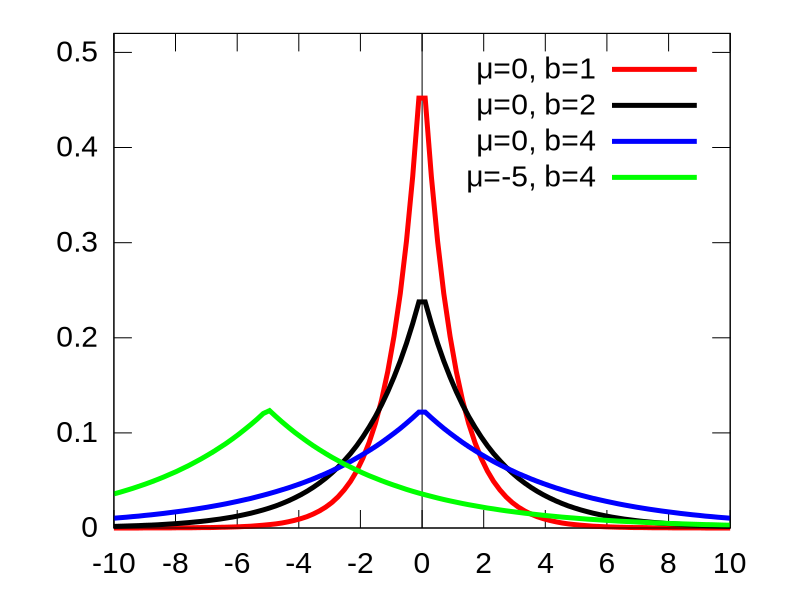
\includegraphics[width=0.6\linewidth]{figures/Laplace_pdf.pdf}
\end{figure}

\end{frame}

\begin{frame}{Achieving Pure DP: The Laplace Mechanism}

\begin{columns}[c]

\begin{column}{.5\textwidth}

\begin{block}{Laplace Mechanism}
$f: D^n \rightarrow \mathbb{R}^k$

$M(D) = f(D) + (Y_1, \dots, Y_k)$

$Y_i \underset{i.i.d}{\sim} \text{Lap}(\frac{\Delta^{(f)}}{\varepsilon})$
\end{block}

Add noise to each coordinate, proportional to the L1 sensitivity

\begin{block}{Example: Sum query}
$f = \sum X_i$, $\Delta^{(f)} = 1$, $k=1$

$\tilde{p} = f(x) + \text{Lap}(\frac{1}{\varepsilon})$
\end{block}

\end{column}

\begin{column}{.5\textwidth}

\begin{table}[]
    \centering
    \begin{tabular}{c|c}
    Name    &   Smokes?\\
    \hline
    Alice     &  0\\
    Bob     & 0\\
    Clair     & 1\\
    $\vdots$    & $\vdots$\\
    Zane    &   1\\
    \end{tabular}
\end{table}

\end{column}
\end{columns}

\end{frame}

\begin{frame}{Privacy Loss Random Variable}

For mechanism $M: D^n \rightarrow Y$ and neighboring datasets $D$, $D'$, we can define the \textbf{privacy loss random variable} $\mathcal{L}_{M(D) || M(D')}$

\vspace{5mm}

\begin{block}{Privacy Loss Random Variable}
  $\mathcal{L}_{M(D)||M(D')} = \ln (\frac{M(D) = \xi}{M(D') = \xi})$, distributed by drawing $\xi \sim M(D)$
\end{block}

\end{frame}


\begin{frame}{Privacy Loss Random Variable}

We can translate between this privacy loss random variable and our $\varepsilon$-DP:
\begin{itemize}
    \item[] $|\mathcal{L}_{M(D) || M(D')}| \leq \varepsilon$ w.p. $1$, for all $D$ and $D'$ neighboring datasets
\end{itemize}

\begin{columns}[T]

\begin{column}{.5\textwidth}

\begin{figure}
    \centering
    \includegraphics[width=1.1\linewidth]{figures/mech_plot_annotated_flattened.pdf}
\end{figure}

\end{column}

\begin{column}{.5\textwidth}

\begin{figure}
    \centering
    \includegraphics[width=1.1\linewidth]{figures/priv_loss_plot_annotated_flattened.pdf}
\end{figure}

\end{column}
\end{columns}

\end{frame}

\begin{frame}{Properties of DP}

\begin{block}{Properties of DP}
\begin{enumerate}
    \item Closed under post-processing
    \begin{itemize}
        \item If $M: D^n \rightarrow Y$ is $\varepsilon$-DP, and $F: Y \rightarrow Z$ is another randomized mapping, then $F \circ M$ is $\varepsilon$-DP
    \end{itemize}
    \item Group privacy
    \begin{itemize}
        \item If $M: D^n \rightarrow Y$ is $\varepsilon$-DP, and $D$, $D'$ differ in $k$ positions, then for all $S \in \text{Range}(M)$:
        \item[] $Pr[M(D) \in S] \leq \exp (k\varepsilon) Pr[M(D') \in S]$
    \end{itemize}
    \item Basic composition
    \begin{itemize}
        \item If we run $k$ $\varepsilon$-DP algorithms sequentially through our data, the full process will be $k\varepsilon$-DP
    \end{itemize}
\end{enumerate}
\end{block}


\end{frame}


\subsection{Approximate Differential Privacy}

\begin{frame}{Approximate Differential Privacy}

We can `loosen' our privacy guarantees a little

Increase utility, not give up that much privacy

\begin{block}{Idea}
We take our original $\varepsilon$-DP privacy guarantee, and add a `cryptographically small' probability that it will not work
\end{block}

It turns out, this is enough to significantly improve utility of our DP mechanism!

\end{frame}


\begin{frame}{Approximate Differential Privacy}

\textit{For $\varepsilon \geq 0$, mechanism $M$ is $\varepsilon, \delta$-differentially private if}, for all $S \subseteq \text{Range}(M)$, and \textbf{neighboring datasets} $D$ and $D'$:

\begin{block}{Approximate Differential Privacy}
$Pr[M(D) \in S] \leq \exp (\varepsilon) Pr[M(D') \in S] + \delta$
\end{block}

If $\delta = 0$, we go back to our original `pure' DP definition

How about the privacy loss random variable?
\begin{itemize}
    \item[] $|\mathcal{L}_{M(D) || M(D')}| \leq \varepsilon$ w.p. $1 - \delta$, for all $D$ and $D'$ neighboring datasets
\end{itemize}

\end{frame}

\begin{frame}{Approximate Differential Privacy}

What should we set $\delta$ to?

Good rule of thumb: $\delta \ll \frac{1}{n}$, where $n$ is the size of the dataset $D$

\begin{block}{Example $0, \delta$-DP Mechanism}
  $M$: For each $x \in D$, output $x$ w.p. $\delta$, and do nothing w.p. $1 - \delta$
\end{block}

Probability we do not release anyone's data point: $(1 - \delta)^n$

Probability we \textbf{do} release someone's data point: $1 - (1 - \delta)^n$

If $\delta$ is around $\frac{1}{n}$, then this is approximately 1 (as $\delta$ increases, this approaches 1)

\end{frame}

\begin{frame}{Achieving Approximate DP: The Gaussian Mechanism}

How do we achieve the $\varepsilon, \delta$-DP guarantee? --- \textbf{Gaussian Mechanism}

\begin{block}{$l_2$ Sensitivity}
$f: D^n \rightarrow \mathbb{R}^k$

$l_2$-sensitivity of function $f$ is: $\Delta_2^{(f)} = \underset{D, D'}{\max} ||f(D) - f(D')||_2$
\end{block}

\end{frame}


\begin{frame}{Achieving Approximate DP: The Gaussian Mechanism}

Gaussian Distribution: $p(x) = \frac{1}{\sqrt{2\pi \sigma^2}}\exp (-\frac{(x - \mu)^2}{2\sigma^2})$

\begin{figure}
    \centering
    \includegraphics[width=0.7\linewidth]{figures/Normal_Distribution_PDF.pdf}
\end{figure}

\end{frame}

\begin{frame}{Achieving Approximate DP: The Gaussian Mechanism}

\begin{columns}[c]

\begin{column}{.5\textwidth}

\begin{block}{Gaussian Mechanism}
$f: D^n \rightarrow \mathbb{R}^k$

$M(D) = f(D) + (Y_1, \dots, Y_k)$

$Y_i \underset{i.i.d}{\sim} \mathcal{N}(0, 2\ln(\frac{1.25}{\delta})\frac{\Delta_2^2}{\varepsilon^2} )$
\end{block}

Add noise to each coordinate, proportional to the L2 sensitivity

\end{column}

\begin{column}{.5\textwidth}

\begin{table}[t]
    \centering
    \begin{tabular}{c|ccc}
    Name    &   Attr. 1 & Attr. 2 & $\dots$\\
    \hline
    Alice     &  0 & 1 & $\dots$\\
    Bob     & 0 & 1 & $\dots$\\
    Clair     & 1 & 0 & $\dots$\\
    $\vdots$    & $\vdots$ & $\vdots$& $\dots$\\
    Zane    &   1 & 0 & $\dots$\\
    \end{tabular}
\end{table}

\end{column}
\end{columns}

\end{frame}


\begin{frame}{Achieving Approximate DP: The Gaussian Mechanism}

\begin{block}{Example: Sum query with more attributes}
Mechanism: $f = \sum X_i$

$D \in \{0, 1\}^{n \times d}$, where $n$ is the number of individuals and $d$ the number of attributes

Worst case for neighboring datasets $D$, $D'$: $D$'s row has all 1s, $D'$'s row has all 0s

$l_1$-sensitivity: $||\mathbf{1} - \mathbf{0}||_1 = ||\mathbf{1}||_1 = d$

$l_2$-sensitivity: $||\mathbf{1}||_2 = \sqrt{d}$

Laplace: $\tilde{p} = f(x) + \text{Lap}(\frac{d}{\varepsilon})$

Gaussian: $\tilde{p} \approx f(x) + \mathcal{N}(0, (\frac{\sqrt{d}}{\varepsilon})^2)$

\end{block}

\end{frame}

\begin{frame}{Benefits of Approximate DP}

\begin{enumerate}
    \item Scale of added noise can be significantly less (with higher dimensions)
    \item Can improve upon basic composition (more advanced composition techniques)
    \begin{itemize}
        \item If we run $k$ $\varepsilon, \delta$-DP algorithms sequentially through our data, the full process will be \textit{less than} $k\varepsilon, k\delta$-DP (depending on the composition technique)
    \end{itemize}
\end{enumerate}

\end{frame}


\section{Differential Privacy for Machine Learning}

\begin{frame}{Applying DP for ML}

\begin{figure}
    \centering
    \includegraphics[width=0.6\linewidth]{figures/YelpReviews.png}
    \caption{\tiny \url{https://medium.com/analytics-vidhya/performing-sentiment-analysis-on-yelp-restaurant-reviews-962334d6336d}}
\end{figure}

\end{frame}


\begin{frame}{Applying DP for ML}

DP and ML: Instead of privatizing an algorithm, we're privatizing a model

Need to choose a `query' as before (associated with the model, dependent on the dataset)

\begin{figure}
    \centering
    \includegraphics[width=0.65\linewidth]{figures/dp_dl.png}
    \caption{\tiny \url{https://medium.com/bluecore-engineering/differential-privacy-in-the-real-world-f31a5df1398f}}
\end{figure}

\end{frame}

\begin{frame}{DP for ML: DP-SGD}

Most common and widely adopted algorithm in differentially private ML: Differentially Private Stochastic Gradient Descent (DP-SGD)

Can apply directly to model training

The `query' of our DP mechanism: Gradient of the loss function

What's the sensitivity of the gradient?

\end{frame}

\begin{frame}{DP for ML: DP-SGD}

Most common and widely adopted algorithm in differentially private ML: Differentially Private Stochastic Gradient Descent (DP-SGD)

Proposed by \citet{Abadi.et.al.2016.SIGSAC}

Can apply directly to model training

The `query' of our DP mechanism: Gradient of the loss function

What's the sensitivity of the gradient? --- $\infty$...

\end{frame}


\begin{frame}{DP for ML: DP-SGD}

\begin{figure}
    \centering
    \includegraphics[width=0.8\linewidth]{figures/DP-SGD.jpg}
    \caption{\tiny \url{https://ai.facebook.com/blog/introducing-opacus-a-high-speed-library-for-training-pytorch-models-with-differential-privacy/}}
\end{figure}

\end{frame}


\begin{frame}{DP for ML: DP-SGD}

\begin{block}{Algorithm for DP-SGD:}
\begin{enumerate}
    \item Select a `lot' of points
    \begin{itemize}
        \item \textbf{Lot}: A set of data points, where each point is selected with probability $L/n$, where $L$ is the `lot size' and $n$ is the size of the dataset
    \end{itemize}
    \item For each point in the `lot', compute the gradient $g_i = \nabla l (\theta_t, x_i, y_i)$, $\forall i \in \text{lot}$
    \item Clip $g_i$ to $l_2$ ball of radius $C$, then average
    \item Add noise
    \item Step in negative direction of gradient
\end{enumerate}
\end{block}

\end{frame}


\begin{frame}{DP for ML: DP-SGD}

\begin{figure}
    \centering
    \includegraphics[width=0.6\linewidth]{figures/abadi-algo.PNG}
\end{figure}

\end{frame}


\begin{frame}{DP for ML: DP-SGD}

Important points about DP-SGD:
\begin{enumerate}
    \item Use \textbf{Poisson sampling} to select lots (\textbf{not} simply iterate over batches)
    \item Moments accountant: Much better bounds on privacy budget
    \item Clipping can slow down computations
\end{enumerate}

\end{frame}

\begin{frame}{DP for ML: DP-SGD}

\begin{figure}
    \centering
    \includegraphics[width=0.6\linewidth]{figures/moments-accountant.PNG}
    \caption{\citet{Abadi.et.al.2016.SIGSAC}}
\end{figure}

\end{frame}

\begin{frame}{DP for ML: DP-SGD}

\begin{figure}
    \centering
    \includegraphics[width=1.1\linewidth]{figures/dp-sgd-speeds.PNG}
    \caption{\citet{subramani2021enabling}}
\end{figure}

\end{frame}

\begin{frame}{Opacus}

\begin{figure}
    \centering
    \includegraphics[width=1.15\linewidth]{figures/Opacus.PNG}
    \caption{\tiny \url{https://ai.facebook.com/blog/introducing-opacus-a-high-speed-library-for-training-pytorch-models-with-differential-privacy/}}
\end{figure}

\end{frame}

\section{Other Methods in Privacy Research}

\begin{frame}{Other Methods in Privacy: Secure Multiparty Computation}

\begin{block}{Secure Multiparty Computation}
Combining private inputs from multiple people, in order to compute a function, without revealing anyone's input to the rest
\end{block}

\textbf{Encryption}: These numbers are encrypted, nobody knows their own share

\textbf{Shared Governance}: The numbers can only be decrypted if everyone agrees

Main aspects:
\begin{enumerate}
    \item Data remains on a remote machine
    \item Model can be encrypted during training
    \item Multiple data owners privately combining their data
\end{enumerate}

\end{frame}

\begin{frame}{Other Methods in Privacy: Federated Learning}

\begin{figure}
    \centering
    \includegraphics[width=0.85\linewidth]{figures/federated-learning.png}
    \caption{\tiny \url{https://blogs.nvidia.com/blog/2019/10/13/what-is-federated-learning/}}
\end{figure}

\end{frame}

\begin{frame}{Other Methods in Privacy: Homomorphic Encryption}

\begin{figure}
    \centering
    \includegraphics[width=0.9\linewidth]{figures/homomorphic-enc.png}
    \caption{\tiny \url{https://research.aimultiple.com/homomorphic-encryption/}}
\end{figure}

\end{frame}

\fontsize{11pt}{0.5cm}\selectfont
\renewcommand{\bibsection}{}

\begin{frame}[allowframebreaks, fragile]{References}

  \bibliographystyle{plainnat}
  \bibliography{biblio}

\end{frame}

\end{document}
